\documentclass[10pt]{beamer}

\usepackage{xeCJK}

\usepackage[T1]{fontenc}

\usepackage[utf8]{inputenc}

\usetheme{metropolis}
\usepackage{appendixnumberbeamer}

\usepackage{booktabs}
\usepackage[scale=2]{ccicons}

\usepackage{pgfplots}

\usepackage{xspace}

\usepackage{listings}

\lstset{
	basicstyle=\ttfamily,
	escapeinside=||
}

\usepackage{graphicx}

\newcommand{\emptyline}{\vspace{\baselineskip}}

\usepackage{ulem}


\title{程序设计教程}
\subtitle{简易调试技术、函数和数组}
\date{2019-11-01}
\author{唐瑞泽}
\institute{tangruize@smail.nju.edu.cn}

\begin{document}
	
\maketitle

\begin{frame}{目录}
	\setbeamertemplate{section in toc}[sections numbered]
	\tableofcontents[hideallsubsections]
\end{frame}

\section{简易调试技术}\label{sec:简易调试技术}

{
\setbeamertemplate{frame footer}{https://nju-projectn.github.io/ics-pa-gitbook/ics2016/}
\begin{frame}[fragile]{调试公理}
    \begin{quote}
        \begin{itemize}
            \item The machine is always right.
            \begin{itemize}
                \item Corollary: If the program does not produce the desired output, it is the programmer's fault.
            \end{itemize}
            \emptyline
            \item Every line of untested code is always wrong.
            \begin{itemize}
                \item Corollary: Mistakes are likely to appear in the ``must-be-correct'' code.
            \end{itemize}
        \end{itemize}
        \emptyline
        \hspace*{\fill} --jyy
    \end{quote}
\end{frame}
}

\begin{frame}[fragile]{常用的调试技能}
    前面讲了 设置严格的编译选项 和 将输入输出重定向 用于辅助调试, 但并不是真正的调试.
    我们常用的调试技术有哪些呢?
    \begin{itemize}[<+- | alert@+>]
        \item 输出调试 (相信大家都用过了)
        \item 设置断点 (在特定的地方停下来)
        \item 单步执行 (一步步看)
    \end{itemize}
\end{frame}

\begin{frame}[fragile]{手动输出调试(可能是错误示范)}
    \begin{itemize}[<+- | alert@+>]
        \item 不知道我的 bug 代码在干嘛, 看一看不就好了!
        \item (凭感觉)在可能出错的地方加上\texttt{printf()}或\texttt{cout}
        \item (凭感觉)输出有关的变量
        \item 没感觉怎么办?
        \item 加很多\texttt{printf()}
        \item -> 眼花缭乱的输出信息 + 调完还要删的\texttt{printf()}
        \item 改进?
    \end{itemize}
\end{frame}

\begin{frame}[fragile]{手动设置断点和单步调试(可能是错误示范)}
    \begin{itemize}[<+- | alert@+>]
        \item 不知道我的代码会不会走到一个分支, 停一下不就好了!
        \item 在想停的地方加上\texttt{getchar();}
        \item 在每个语句下都加个\texttt{getchar();}就可以单步执行了
        \item -> 非常麻烦 + 破坏输入格式 + 单步执行也难以获取有用信息
        \item 改进?
    \end{itemize}
\end{frame}

\begin{frame}[fragile]{设置断点}
    下载 \href{http://problemoverflow.top/download/function\_array.c}{function\_array.c}
    并将代码添加到一个CLion工程中.
    如果使用gcc编译, 需要添加编译选项 \texttt{-g -Og}
    \begin{itemize}[<+- | alert@+>]
        \item 我们希望程序执行到\texttt{main()}函数时停下
        \item 单击第20行行号右边空白, 产生一个红点 (gdb: \textbf{b}reak)
        \item Shift + F9 或单击调试的图标开始调试
        \begin{figure}[ht!]
            \centering
            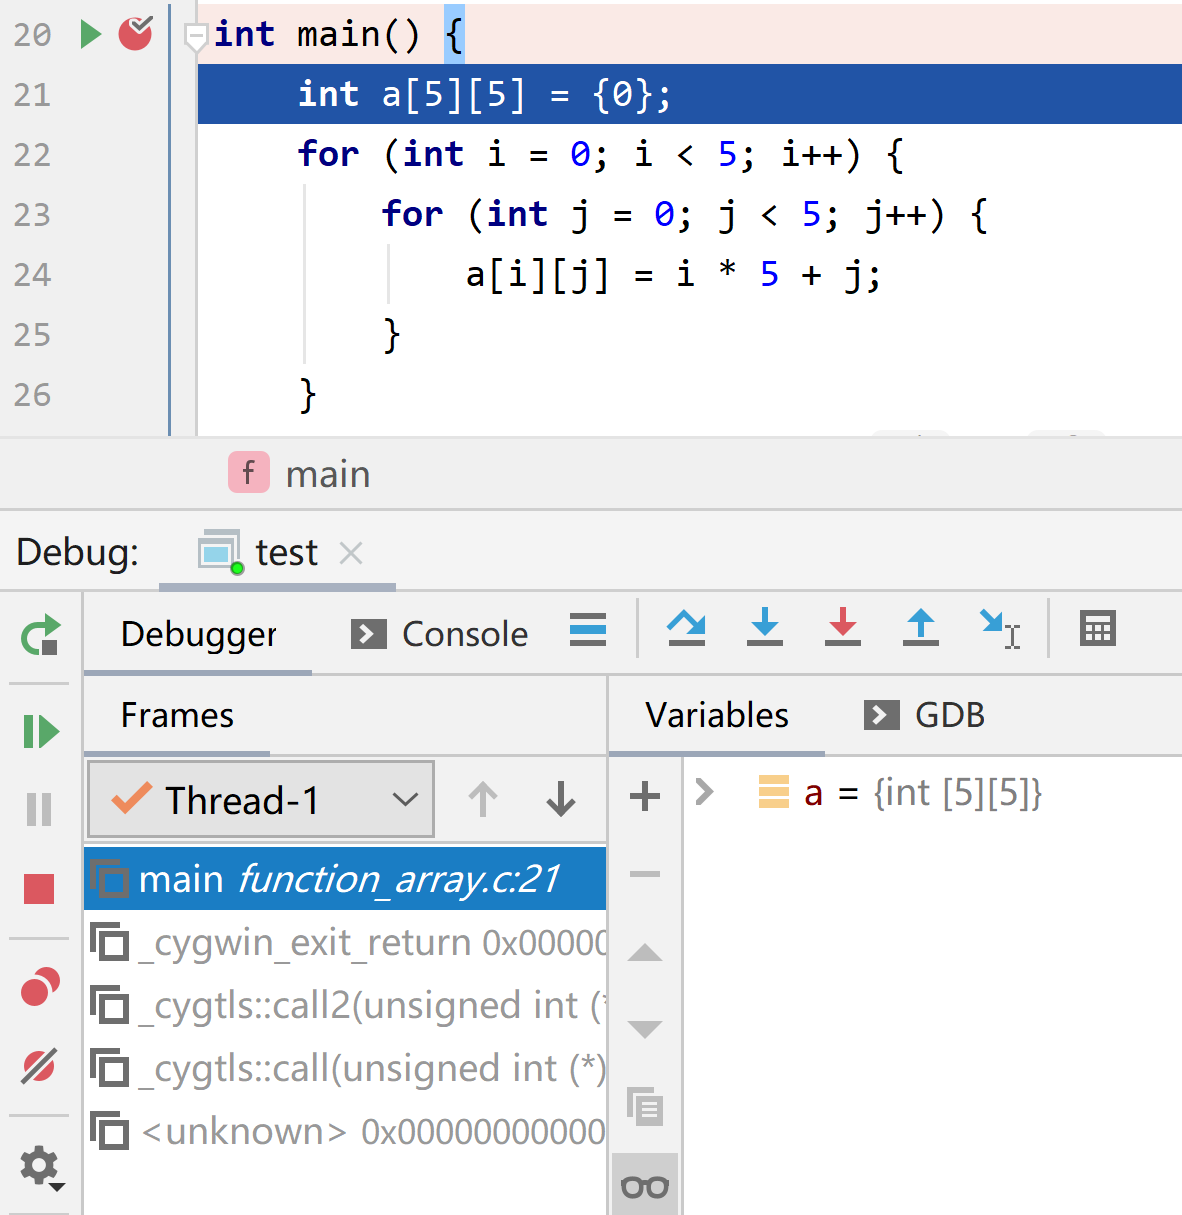
\includegraphics[width=50mm]{figs/clion_b_main.png}
            \caption{在main函数设置断点}
        \end{figure}
    \end{itemize}
\end{frame}

\begin{frame}[fragile]{查看变量信息}
    双击调试窗口Variables的空白处或点击 + 号, 输入你想观察的表达式 (gdb: \textbf{p}rint)
    \begin{figure}[ht!]
        \centering
        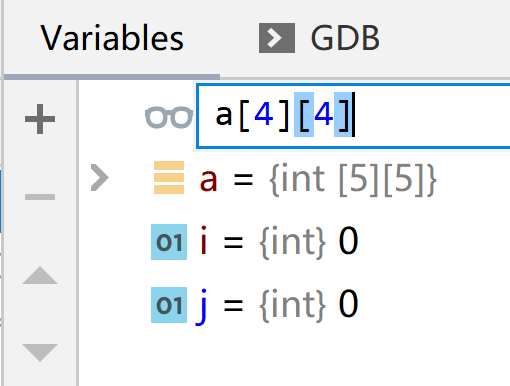
\includegraphics[height=25mm]{figs/clion_new_watch.png}
        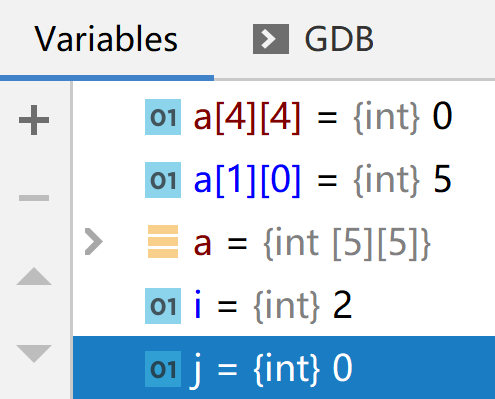
\includegraphics[height=25mm]{figs/clion_new_watch2.png}
        \caption{添加表达式}
    \end{figure}
\end{frame}

\begin{frame}[fragile]{单步执行}
    我们希望程序每次运行一行C语言代码, 便于观察执行那一步时的状态
    \begin{figure}[ht!]
        \centering
        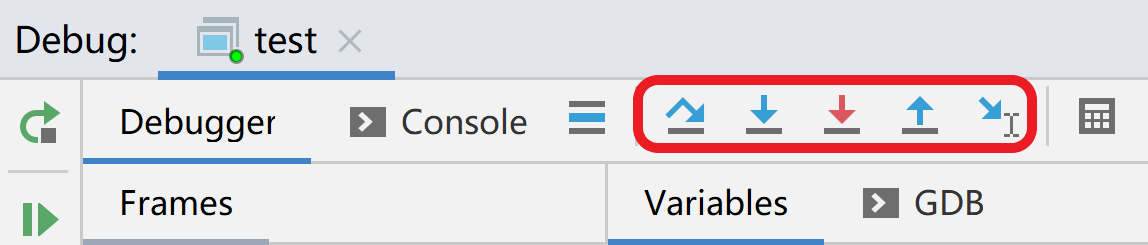
\includegraphics[width=50mm]{figs/clion_step_buttons.png}
        \caption{CLion调试单步执行按钮}
    \end{figure}
    从左到右依次的功能:
    \begin{itemize}[<+- | alert@+>]
        \item Step Over (F8, gdb: \textbf{n}ext): 执行一行C语言语句,  如果该行有函数调用, 函数将被执行完 (不单步进入函数体)
        \item Step Into (F7, gdb: \textbf{s}tep): 同上, 不同之处为会进入函数体
        \item Force Step Into: 同上, 不同之处为会进入标准库函数
        \item Step Out (Shift + F8, gdb: \textbf{fin}ish): 将当前的函数执行至结束
        \item Run to Cursor (Alt + F9): 执行到鼠标指针的位置
    \end{itemize}
\end{frame}

\begin{frame}[fragile]{添加监视点}
    我们希望程序能在某些条件满足的情况下停下, 比如变量被修改, 等于某个值, 大于某个值, 小于另一个变量等等
    \begin{itemize}[<+- | alert@+>]
        \item 先使用查看变量信息的方法添加你感兴趣的表达式
        \item 在该表达式上右键 - Add Watchpoint (gdb: watch)
        \item 查看监视点 (gdb: info watchpoints 或 info breakpoints)
        \begin{figure}[ht!]
            \centering
            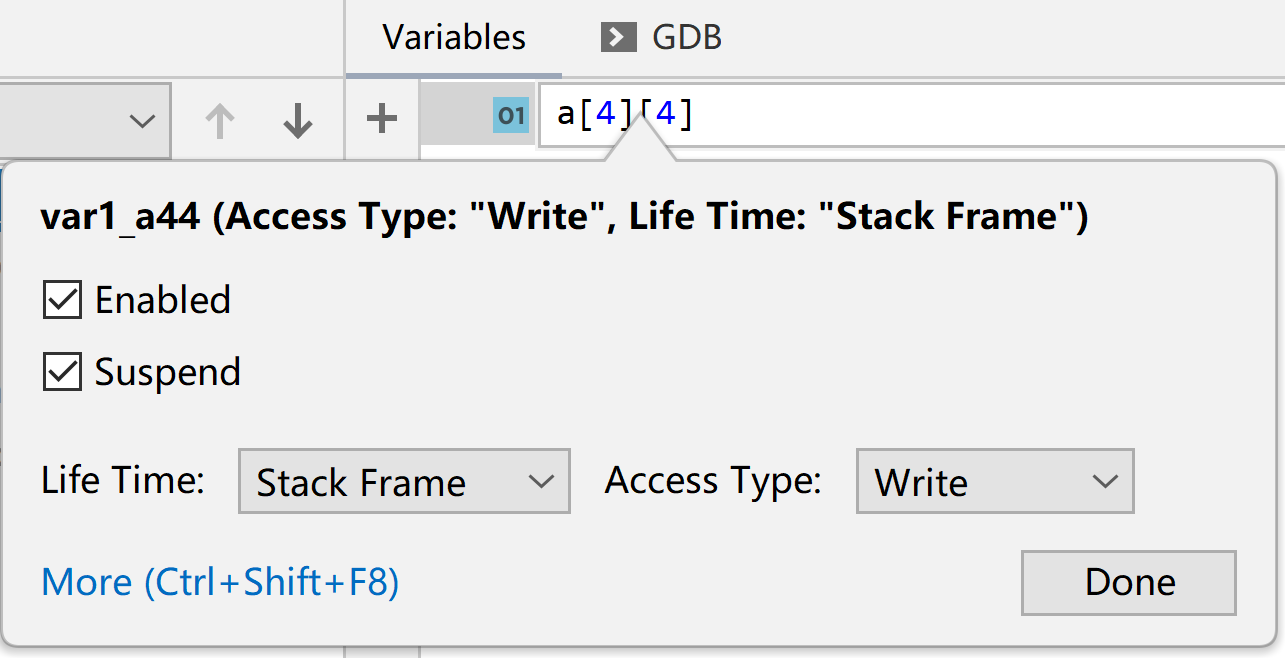
\includegraphics[height=25mm]{figs/clion_watchpoint.png}
            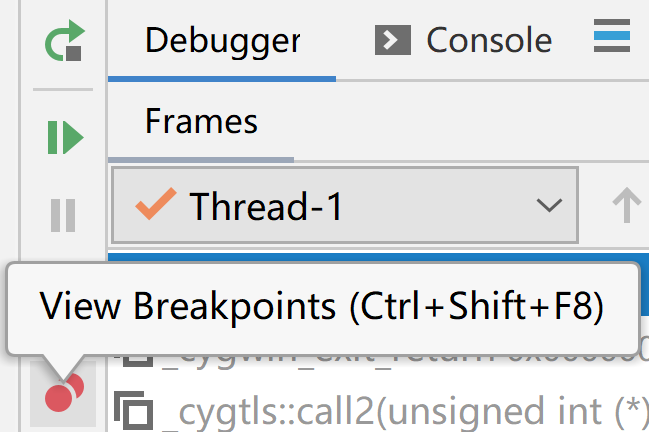
\includegraphics[height=25mm]{figs/clion_info_watchpoint.png}
            \caption{CLion添加和查看监视点}
        \end{figure}
    \end{itemize}
\end{frame}

\begin{frame}[fragile]{查看调用链}
    \texttt{main()}调用了\texttt{printSumArray()}.
    而执行到\texttt{printSumArray()}时, 我们希望查看\texttt{main()}的变量状态.
    \begin{itemize}[<+- | alert@+>]
        \item 每个函数调用是一个栈帧, CLion的Frames窗口有栈帧信息 (gdb: \textbf{b}ack\textbf{t}race)
        \item 点击其他的栈帧可以切换 (gdb: \textbf{f}rame)
        \begin{figure}[ht!]
            \centering
            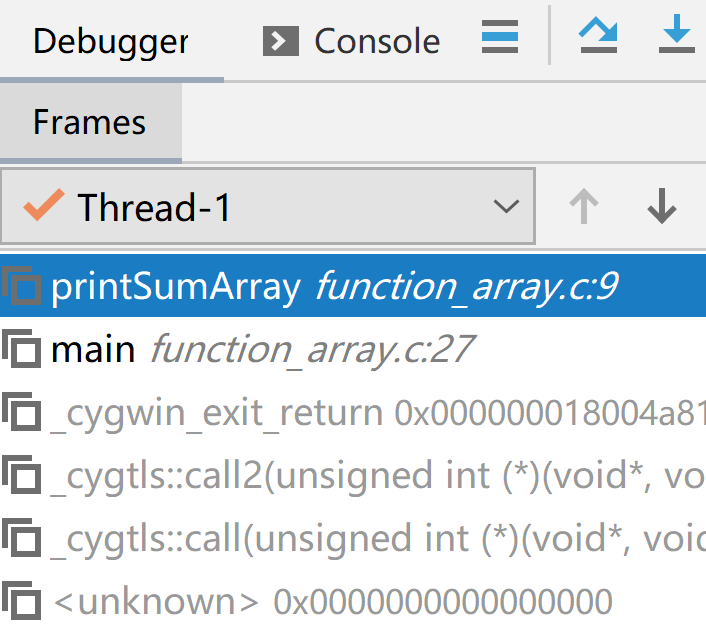
\includegraphics[width=40mm]{figs/clion_frame.png}
            \caption{CLion查看栈帧链}
        \end{figure}
    \end{itemize}
\end{frame}

\begin{frame}[fragile]{使用GDB}
    打开CLion调试的GDB窗口, 或使用命令行 \textbf{gdb ./main.exe}

    \begin{table}[]
        \begin{tabular}{|l|l|}
            \hline
            \textbf{行为} & \textbf{命令} \\ \hline
            设置断点在\texttt{main()} & \texttt{b main} \\ \hline
            设置断点在第八行 & \texttt{b 8} \\ \hline
            运行程序 & \texttt{r} \\ \hline
            继续执行 & \texttt{c} \\ \hline
            查看变量a[4][4] & \texttt{p a[4][4]} \\ \hline
            单步不进入函数执行3行 & \texttt{n 3} \\ \hline
            单步进入函数执行1行 & \texttt{s} \\ \hline
            执行当前函数至返回 & \texttt{fin} \\ \hline
            当a[4][4]的值改变时停下 & \texttt{watch a[4][4]} \\ \hline
            当a[3][3]的值不等于0时停下 & \texttt{watch a[3][3] != 0} \\ \hline
            查看断点 & \texttt{info breakpoints} \\ \hline
            查看栈帧链 & \texttt{bt} \\ \hline
            选择栈帧\#1 & \texttt{f 1} \\ \hline
        \end{tabular}
        \caption{GDB常用命令一览表}
    \end{table}
\end{frame}

\section{函数}\label{sec:函数}

\begin{frame}[fragile]{函数定义}
    通过OJ的练习的联系, 相信大家对函数已经比较熟悉.

    函数结构: \texttt{type name (para1, para2, \ldots) \{ statements \}}

    \begin{itemize}[<+- | alert@+>]
        \item \texttt{type}: 返回值的类型, 没有返回值为\texttt{void}
        \item \texttt{name}: 函数名, 命名规则与变量名相同
        \item \texttt{paras}: 参数列表, 每个参数包含类型和参数名, 用逗号分隔.
        没有参数可以留空, 或用\texttt{void}显式表示参数列表为空
        \item \texttt{statements}: 函数体, 被大括号包围
        \item 举例:
        \begin{lstlisting}[language=c]
int addition(int a, int b) {
    return a + b;
}
        \end{lstlisting}
    \end{itemize}
\end{frame}

\begin{frame}[fragile]{函数调用}
    函数调用需使用与被调用函数匹配的参数列表

    如果函数有返回值, 可以赋值给匹配的类型, 也可以忽略

    \emptyline
    \begin{lstlisting}[language=c]
int z = addition(5, 3);
    \end{lstlisting}
\end{frame}

\begin{frame}[fragile]{函数声明}
    如果有多个源代码文件, 或同一文件中函数调用在函数实现之前,
    则编译器看不到被调用函数的信息(参数类型个数, 返回值), 无法进行编译

    这种情况下, 可以对函数进行声明

    函数声明就像把函数体去掉, 换成分号, 比如:
    \begin{lstlisting}[language=c]
int addition(int a, int b);
    \end{lstlisting}

    头文件中应只有声明, 没有定义 (否则一个程序包含多次该头文件将出现重定义错误)
\end{frame}

\begin{frame}[fragile]{递归函数}
    函数可以调用其自身, 隐式地维护了一个栈(后进先出的数据结构), 对有的任务而言非常方便

    如果能用循环实现, 且不需要维护栈的信息, 通常循环效率更高
    \begin{columns}[T,onlytextwidth]
        \column{0.40\textwidth}
        \scriptsize
        \begin{lstlisting}[language=c]
unsigned short
factorial (unsigned short a) {
    if (a > 1)
        return a * factorial(a-1);
    else
        return 1;
}
        \end{lstlisting}

        \column{0.10\textwidth}
        \column{0.50\textwidth}
        \scriptsize
        \begin{lstlisting}[language=c]
unsigned short
factorial_loop(unsigned short a) {
    unsigned short result = a;
    while (--a)
        result *= a;
    return result;
}
        \end{lstlisting}
    \end{columns}

    分别传入参数 -1 调用这两个函数, 会发生什么?
\end{frame}

\section{数组}\label{sec:数组}

\begin{frame}[fragile]{数组定义}
    数组是一系列相同类型元素, 放置在一片连续的内存区域.
    每个元素都能单独被索引到

    定义方式: \texttt{type name [elements][elements];}

    \begin{itemize}[<+- | alert@+>]
        \item \texttt{type}: 数组类型
        \item \texttt{name}: 变量名
        \item \texttt{elements}: 元素个数
        \item 注意数组元素索引从0开始, 最大索引为 elements-1
    \end{itemize}
\end{frame}

\begin{frame}[fragile]{数组初始化}
    \begin{lstlisting}[language=c]
    int foo [5];
    int foo [5] = { 16, 2, 77, 40, 12071 };
    int bar [5] = { 10, 20, 30 };
    int baz [5] = { 0 };
    int foo [] = { 16, 2, 77, 40, 12071 };
    \end{lstlisting}

    \begin{itemize}[<+- | alert@+>]
        \item 第1行, 数组大小为5, 不对数组进行初始化, 可能是随机值, 不能在赋值前使用
        \item 第2行, 数组大小为5, 所有元素都提供了初值
        \item 第3行, 数组大小为5, 只提供了一部分初值, 其他的, 即 bar[3] 和 bar[4] 将被初始化为0
        \item 第4行, 数组大小为5, 所有元素都被初始化为0
        \item 第5行, 数组大小根据初始化提供的初值个数确定, 即5.
        如果提供了所有的初值或不需要显式指定元素个数时, 这种初始化比第2行好
    \end{itemize}
\end{frame}

\begin{frame}[fragile]{多维数组}
    多维数组可以当作是数组的数组, 比如 \texttt{int a[5][5];}

    但本质上仍然是一片连续的内存区域, \texttt{int a[5][5];} 等价于 \texttt{int b[25];}

    获取\texttt{a[3][4]} 等价于 \texttt{b[19]}, 如果两个维度不相同, 如果有三个维度, 你知道怎么算吗?
\end{frame}

\begin{frame}[fragile]{数组作为函数参数}
    \begin{itemize}[<+- | alert@+>]
        \item 函数参数格式: \texttt{type name[][elements][elements]}
        \item 即除了第一维大小可省略 , 其他维度都要给定大小
        \item 思考为什么要这样做, 与前面说的多维数组和一维数组等价表示有什么关系?
        \item 举例 \\
        函数声明为: \texttt{void procedure(int arg[][3], int n);}\\
        调用该函数: \texttt{procedure(a, 5);}
    \end{itemize}
\end{frame}

\begin{frame}[standout]
	Questions?
\end{frame}

\end{document}
